A perturbációszámítás a Green-függvény egyik legjelentősebb alkalmazása. Ebben a részben a Green-függvény perturációs sorának a konvergencia tulajdonságait vizsgáljuk. A konvergencia tartományát és sebességét befolyásolja a perturbáló operátor triviális módosítása, konkrétan a vizsgált példában az $\frac{FL}{2}\op{I}$ operátort a perturbáló tagból levonjuk és a perturálatlan operátorhoz hozzáadjuk. Ezzel a teljes Hamilton operátor nem változik, de a perturbációs sor konvergenciája igen.

A perturbációszámításhoz a Hamilton operátort két részre bontjuk,
\begin{equation}
	\op{H} = \op{H}_0 + \op{V}.
\end{equation}
A $\op{H}_0$ operátorhoz tartozó rezolvens operátor $\op{G}_0\left(E\right)$. Mind $\op{H}$ és mind $\op{H}_0$ kifejezhetőek a rezolvenseikkel, ha ezeket behelyettesítjük a fenti egyenletbe, implicit egyenletet kapunk $\op{G}\left(E\right)$-re nézve,
\begin{equation}
	-\op{G}^{-1}\left(E\right) + E = -\op{G}_0^{-1}\left(E\right) + E + \op{V}.
\end{equation}
Ezt kisebb átalakítások után fel lehet használni perturbációszámításra. Az egyenletet balról $\op{G}_0\left(E\right)$-vel, jobbról $\op{G}\left(E\right)$-vel szorozzuk, így
\begin{equation}
	\op{G}\left(E\right) = \op{G}_0\left(E\right) + \op{G}_0\left(E\right)\op{V}\op{G}\left(E\right)
	\label{green:pertmaster}
\end{equation}
eredményhez jutunk, ami a Dysonegyenletnek felel meg. Megfelelően definiálva $\op{G}_n\left(E\right)$ operátorokat,
\begin{equation}
	\op{G}_n\left(E\right) = \op{G}_0\left(E\right)\sum_{k=0}^n\left(\op{V}\op{G}_0\left(E\right)\right)^k,
\end{equation}
a $\op{G}_n$-ekre \aeqref{green:pertmaster} egyenlethez hasonló rekurziós összefüggés áll fent,
\begin{equation}
	\op{G}_{n+1}\left(E\right) = \op{G}_0\left(E\right) + \op{G}_0\left(E\right)\op{V}\op{G}_n\left(E\right).
	\label{perturbation:rekurzió}
\end{equation}
Ha $\norm{\op{V}\op{G}_0\left(E\right)} < 1$ akkor a $\op{G}_n$ sorozat konvergál. Operátor normának a Hilbert-tér normája által indukált normát vesszük, így az operátorok konvergenciája kompatibilis a Hilbert-tér beli konvergenciával.
\begin{equation}
	\norm{\op{A}}=\sup \Set{\sqrt{\Braket{\phi|\op{A}^\dagger \op{A}|\phi}} \text{, ahol} \Braket{\phi|\phi}=1}.
\end{equation}
A sor határértéke \aeqref{perturbation:rekurzió} miatt kielégíti \aeqref{green:pertmaster} egyenletet. Így konvergencia esetén
\begin{equation}
	\op{G}\left(E\right) = \op{G}_0\left(E\right)\sum_{n=0}^\infty\left(\op{V}\op{G}_0\left(E\right)\right)^n.
	\label{perturbation:series}
\end{equation}
Ez azt jelenti, hogy ha egy operátornak van projektor felbontása, akkor a normája a legnagyobb sajátérték abszolút értéke lesz, vagy általános esetben a sajátértékek szuprémuma. Ez hasznos jelen esetben is, mivel így meg tudjuk határozni az $\op{V}=a\op{x}+b$ operátor normáját. Ennek az operátornak a sajátfüggvényei a $\delta(x-x_0)$ függvények, így a sajátértékek maximuma a $[0,L]$ tartományban
\begin{equation}
	\norm{\op{V}}=\max(\rvert b \lvert, \lvert aL+b\rvert).
\end{equation}
\Aeqref{green:greensum} egyenlet alapján $\op{G}(E)$ normája is meghatározható, az összeg nevezői közül kiválasztva a legkisebb abszolút értékűt,
\begin{equation}
	\norm{\op{G}(E)}=\frac{1}{\lvert E-E_k\rvert},
\end{equation}
ahol $E$-hez a komplex síkon a legközelebbi sajátérték $E_k$. Ezek segítségével felső korlátot lehet adni a $\norm{\op{G}_1\op{V}}$-re.

A Hamilton-operátort eredetileg
\begin{equation}
	\begin{aligned}
		\op{H}=&\frac{\op{p}^2}{2m}+F\op{x}=\op{H}_1+\op{V}_1\\
		\op{H}_1=&\frac{\op{p}^2}{2m}\\
		\op{V}_1=&F\op{x}\\
		\op{G}_{01}(E)&=\frac{1}{E-\op{H}_1}
	\end{aligned}
\end{equation}
részekre bontottuk. Ebben ha az esetben a $\op{G}_{01}$ pólusaitól legalább $FL$ távolságban, azaz $\rvert E-E_k\lvert>FL$, a komplex energia síkban a sor garantáltan konvergál, mert
\begin{equation}
	\norm{\op{G}_{01}(E)V_1}<\norm{\op{G}_{01}(E)}\norm{\op{V}_1}=\frac{FL}{\rvert E-E_k\lvert}<1.
\end{equation}
Vizsgálunk egy módosított felontást is,
\begin{equation}
	\begin{aligned}
		\op{H}=&\frac{\op{p}^2}{2m}+\frac{FL}{2}+F\op{x}-\frac{FL}{2}=\op{H}_2+\op{V}_2\\
		\op{H}_2=&\frac{\op{p}^2}{2m}+\frac{FL}{2}\\
		\op{V}_2=&F\op{x}-\frac{FL}{2}\\
		\op{G}_{02}(E)&=\frac{1}{E-\op{H}_2}
	\end{aligned}.
\end{equation}
A perturbációszámítás során így a perturbálatlan operátor szerepét a $\frac{\op{p}^2}{2m}+\frac{FL}{2}$ operátor tölti be.
Ebben az esetben a garantált konvergencia tartomány nagyobb, az $\left\lvert E-E_k-\frac{FL}{2}\right\rvert > \frac{FL}{2}$ reláció teljesülése esetén a perturbációs sor garantáltan konvergál,
\begin{equation}
	\norm{\op{V}_{02}\op{G}_2(E)}<\norm{\op{V}_2}\norm{\op{G}_{02}(E)}=\frac{\frac{FL}{2}}{\left\lvert E-E_k-\frac{FL}{2}\right\rvert}<1.
	\label{perturbation:convradius}
\end{equation}
A második sorhoz tartozó perturbálatlan Green-függvény
\begin{equation}
	\op{G}_{02}(E)=\frac{1}{E-\left(\frac{\op{p}^2}{2m}+\frac{FL}{2}\right)}=\op{G}_{01}\left(E-\frac{FL}{2}\right),
\end{equation}
könnyen kifejezhető az eredeti eset perturbálatlan $\op{G}_1$ Green-függvényével.

A $\frac{\op{p}^2}{2m}$ Green-függvénye a $[0,L]$ tartományban \aref{egzakt}. fejezethez hasonlóan meghatározható,
\begin{equation}
	G_1\left(x,y;E\right) = -\frac{\hbar}{\sqrt{2m}}\frac{1}{\sin\left(kL\right)}\times
	\begin{cases}
		\sin\left(k\left(y-L\right)\right)\sin\left(kx\right) & x\leq y\\
		\sin\left(k\left(x-L\right)\right)\sin\left(ky\right) & x\geq y\\
	\end{cases},
\end{equation}
\begin{equation}
	k = \frac{\sqrt{2mE}}{\hbar}.
\end{equation}

A $G_01(x,y;E)$ diszkretizálásával lehetővé válik a perturbációs sor numerikus kiértékelése. A $[0,L]$ tartományból $N$ egyenletes eloszlású pontot választva, az operátorok közelíthetőek $N\times N$ mátrixokkal, és az operátorok szorzata a közelítő mátrixok szorzatával,
\begin{equation}
	\begin{aligned}
		x_k&=\frac{kL}{N-1}\\
		\op{A}&\rightarrow A_{kl}=\Braket{x_k|\op{A}|x_l}\\
		\op{A}\op{B}&\rightarrow (AB)_{kl}=\frac{L}{N-1}\sum_{m=0}^{N-1}A_{km}B_{ml}
	\end{aligned},
\end{equation}
az indexek $0,1,\dots N-1$ értékűek lehetnek. Szükség van még a operátor norma közelítésére is. A standard $\ell^2$ mátrixnorma megszorozva $\frac{L}{N-1}$-el megfelelő. A skálázási faktorra azért van szükség, mert az operátorok szorzatának közelítésében a mátrix szorzat is skálázva van. A két különböző perturbáció és a különböző $N$ esetek konvergenciája numerikusan vizsgálható,
\begin{equation}
	(V_1G_1(E))_{kl}=Fx_kG_1(x_k,y_l,E)
\end{equation}
az első perturbációs sorban felmerülő $\op{V}\op{G}_0(E)$ mátrix közelítése,
\begin{equation}
	\left(V_2G_2(E)\right)_{kl}=F\left(x_k-\frac{L}{2}\right)G_1\left(x_k,y_l;E-\frac{FL}{2}\right)
\end{equation}
pedig a módosított perturbációs sorban felmerülő $\op{V}_2\op{G}_2(E)$ operátor mátrix közelítése. Minden eszköz adott, hogy a $\norm{\op{G}_n(E)-\op{G}(E)}$ sorozatot a diszkretizáció segítségével numerikusan vizsgáljuk. Az eredményeket \aref{perturbation:covergencerate}. ábra mutatja. Látható, hogy adott finomságú diszkretizáció esetén a második perturbációs sor, ami a $V(x)=Fx-\frac{FL}{2}$ potenciálhoz tartozik, gyorsabban közelít az egzakt Green-függvényhez. A gyorsabb konvergencián túl amikor a numerikusan kiértékelt sor stacionáriussá válik a lépésszám függvényében, a kapott eredmény közelebb van az egzakt Green-függvényhez. Ez a különbség, amelyik tetszőleges lépésszám után is megmarad, a diszkretizáció finomságával jó közelítéssel fordítottan arányos, az ábrán a felbontás duplázása a különbség normájának logaritmusát egy állandó értékkel csökkentette.
\begin{figure}[H]
	\centering
	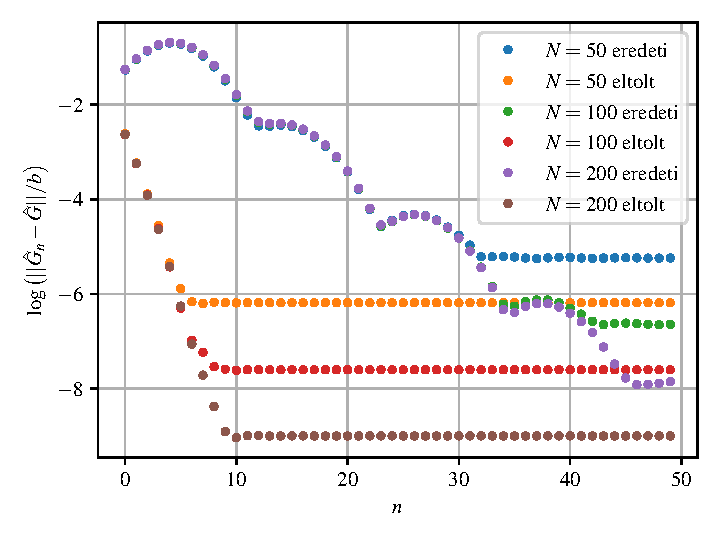
\includegraphics[scale=1]{./figs/convergencerate.pdf}
	\caption[A Green-függvény perturbációs sorának konvergencia sebessége]{Az ábra a $\op{G}_n$ sorozat és az egzakt $\op{G}$ operátor távolságát vizsgálja. A doboz mérete $aL=7$, és az energia $bE=6.5+4i$. A függőleges tengely logaritmikus, hogy a exponenciális csökkenés könnyen látható legyen. Mind az eredeti, $V=Fx$, és módosított, $V=Fx-\frac{FL}{2}$, perturbáló potenciálból származtatott sor konvergenciája ábrázolva van különböző finomságú diszkretizációk, azaz $N$ esetén.}
	\label{perturbation:covergencerate}
\end{figure}
Mivel \aref{perturbation:covergencerate}. ábrán a lépésszám függvényében a különbség normája exponenciálisan csökken amíg el nem ér egy a diszkretizáció finomságától függő minimális hibát, a konvergencia vagy divergencia sebességét meg lehet becsülni a lépések függvényében a normákra illesztett exponenciális függvény kitevőjével,
\begin{equation}
	d(n) = d(0)\exp(-\alpha n)+r,
	\label{perturbation:fit}
\end{equation}
ahol $\alpha$ jelentése a konvergencia sebessége, ha negatív, a sor divergál, $d$ pedig a egzakt eredménytől való eltérés operátor normája. A maradék tagot $r$ modellezi, ez az $r$ tag lesz közelítőleg fordítottan arányas $N$-nel. 
\begin{figure}[H]
	\centering
	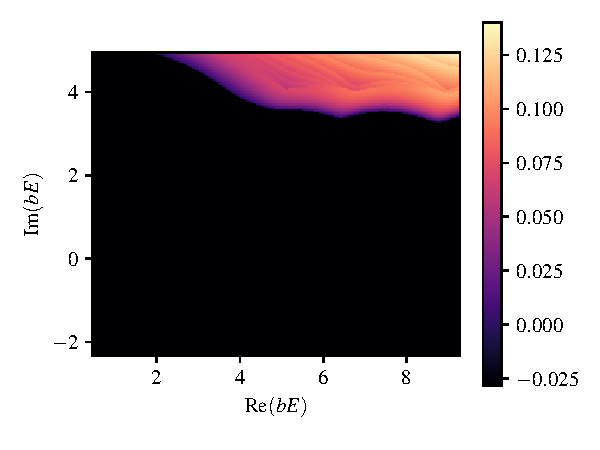
\includegraphics[scale=1]{./figs/convergenceOriginal.pdf}
	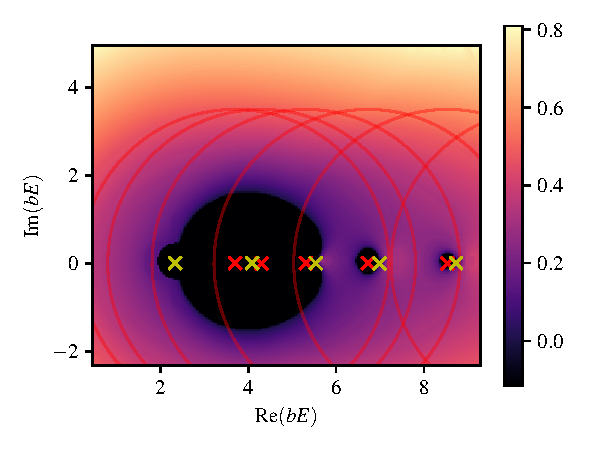
\includegraphics[scale=1]{./figs/convergenceImproved.pdf}
	\caption[A Green-függvény perturbációs sorának konvergenciatartománya]{Ez az ábra a két perturbációs sor konvergenciáját hasonlítja össze a komplex energia síkon. Mind a két ábrán a doboz mérete $aL=7$. A felső ábra a $V=Fx$ perturbáló potenciálnak, míg az alsó a $V = Fx-FL/2$ perturbáció szerinti sornak felel meg. A fekete tartományok divergenciát jelölnek, míg a többi szín a sorfejtés tagjainak csökkenési sebességét jellemzik az $\alpha$ paraméterrel \aeqref{perturbation:fit} egyenletből. A piros körökön kívüli tartomány \aeqref{perturbation:convradius} formula által garantált konvergencia tartományt jelöli. A piros x-ek a $\hat{G}_0$ pólusait, a sárga x-ek pedig az egzakt $\hat{G}$ operátor pólusait jelölik.}
	\label{perturbation:convergencerange}
\end{figure}
\Aref{perturbation:convergencerange}. ábra jól mutatja, hogy a második perturbációs sor gyorsabban, és nagyobb tartományban konvergál. A két perturbációs sor között a különbség csupán annyi, hogy a perturbáló tag egy triviális részét, az egység operátorral arányosat, a perturbálatlan Hamilton-operátorhoz csoportosítjuk a perturáló operátorból, ezzel csökkentve a $\op{V}\op{G}_0(E)$ normáját \aeqref{perturbation:series} egyenletben.






